
\documentclass{article}

%%%%%%%%%%%%%%% LIBRERIAS %%%%%%%%%%%%%%%%%%%%%
\usepackage{amsmath}
\usepackage{titlesec}
\usepackage{titletoc}
\usepackage{graphicx}
\usepackage[spanish,es-tabla]{babel} % 'es-tabla' cambia Cuadro→Tabla
\usepackage{hyperref}                % cargar después de babel
\usepackage{float}
%%%%%%%%%%%%%%%%%%% VARIABLES %%%%%%%%%%%%%%%%%%%%
\newcommand{\Facultad}{Instituto Tecnológico \\de\\ Buenos Aires} %constantes
\newcommand{\TPn}{Trabajo Práctico N° 1}
\newcommand{\TPtema}{Corriente Continua}
\renewcommand{\thesection}{\arabic{section}}          % 2
\renewcommand{\thesubsection}{\quad \alph{subsection}}   % a
\renewcommand{\thesubsubsection}{\quad \thesubsection.~\roman{subsubsection}} % a. i
\graphicspath{{imagenes&matlab/}} %para que acceda a las fotos en la carpeta directamente


%%%%%%%%%%%%%%%%%% FORMATO TÍTULO Y NUMERACIÓN %%%%%%%%%%%%%%%%%%%
% Numeración de secciones
\renewcommand{\thesection}{\arabic{section}.}          
\renewcommand{\thesubsection}{\thesection\arabic{subsection}}       
\renewcommand{\thesubsubsection}{$\alph{subsubsection})$}

% Numerar hasta subsubsecciones
\setcounter{secnumdepth}{3}

% Formato de títulos
\titleformat{\section}{\Huge\bfseries}{\thesection}{1em}{}
\titleformat{\subsection}{\LARGE\bfseries}{\thesubsection}{0.5em}{}
\titleformat{\subsubsection}{\large\bfseries}{\thesubsubsection}{0.5em}{}



%%%%%%%%%%%%%%%%%%% ARCHIVO %%%%%%%%%%%%%%%%%%%%%%%%
\begin{document}

    %%%CARATULA%%%
    \begin{titlepage} %creo portada

        \begin{flushleft}
            \centering
            
\includegraphics[width=0.3\textwidth]{Logo_ITBA.png}
        \end{flushleft}

        \centering
            
        {\scshape\LARGE \Facultad \par} %\par sirve para indicar un final de parrafo
        \vspace{1cm}                    %esto hace un espacio entre lineas de 1cm


        {\huge\bfseries \TPn \par}
        \vspace{1.5cm}
        {\Large Teoría de Circuitos I\\ 25.10 \par}
        \vfill                      %sirve para rellenar el espacio y quede simétrico. Si se añaden otros, se dividen el espacio de forma equitativa
        {\Large \bfseries Grupo N° 5 \par}
        \vspace{1cm}
        {\large Juan Bautista Correa Uranga \hfill Legajo: 65016 \par} %\hfill sirve para hacerlo simétrico
        {\large Juan Ignacio Caorsi \hfill Legajo: 65532  \par}
        {\large Rita Moschini \hfill Legajo: 67026 \par} 
        \vfill
        {\large \today\par}
        \vfil

    \end{titlepage}


    %%%RESUMEN%%%
    {\centering \LARGE \bfseries Resumen \par}
        Este trabajo práctico consiste de dos partes, la primera teniendo como objetivo verificar los análisis de Thevenin y Norton para el estudio
        de circuitos, y la segunda buscando comprobar la máxima transferencia de potencia para el valor de resistencia de Thevenin/Norton correspondiente. \par
        

        En la primera parte de la práctica se ensambló el circuito indicado por la consigna con los nodos A y B formando un circuito abierto. Luego, se
        realizaron las mediciones de la tensión de Thevenin y la corriente de Norton entre los mismos, así como la resistencia de Thevenin/Norton. 
        Se considera que los resultados medidos durante la práctica ($V_{Th} = 9,29V$, $I_{Nt} = 24,6 mA$ y $R_{Th/Nt} = 388 \Omega$) son suficientemente 
        semejantes a los teóricos ($V_{Th} = 9,25 V$, $I_{Nt} = 25,19 mA$ y $R_{Th/Nt} = 367,1436 \Omega$) como para considerarlos coherentes con lo 
        estudiado en las teóricas de la materia.  \par

        En la segunda parte de la práctica se conectó una resistencia variable entre los nodos A y B y se fue aumentando su valor de entre su mínimo 
        ($0 \Omega$) y su máximo ($500 \Omega$), a la vez que se medían con cada variación de la resistencia el valor de la misma, la caida de
        tensión entre los nodos A y B y la corriente que circulaba en aquella rama. Para visualizar la semejanza entre los resultados teóricos y los 
        prácticos, se recomienda ver la figura \ref{fig:graficoTransferenciaPotencia}, la cual muestra que los valores medidos en su mayoría se asemejan
        satisfactoriamente a los previstos teóricamente. \par



    \newpage

    %%%INDICE%%%
    \tableofcontents %esto sirve para crear el índice
    \newpage

    %%%Introduccion%%%
    \section{Introducción}

    %%%Desarrollo%%%
    \indent
    \section{Desarrollo}
        \quad Para el desarrollo de este trabajo, se consideró el circuito indicado en la esquemática \autoref{fig:esquemática}.\par
        Para construirlo se usaron los siguientes materiales:\par
        
            	\begin{itemize}
                \item $V_{S_{1}}$ = 12 V
                \item $V_{S_{2}}$ = 5 V
                \item $R_{1} = R_{2} = 220 ~\Omega $
                \item $R_{3} = 680~ \Omega $
                \item $R_{4} = 100~ \Omega $
                \item Resistencia variable con $R_{L_{max}} = 500~\Omega$
                \item Protoboard y cables puentes
                \end{itemize}
        
        
        Primero, se procedió a la construcción del circuito según lo indicado por la esquemática \autoref{fig:esquemática}.\par %falta añadir foto

\begin{figure}[!h]
  \centering
  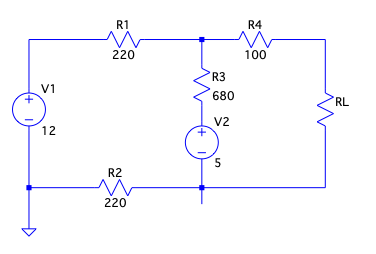
\includegraphics[width=0.5\textwidth]{circuitoLTSpice.png}
  \caption{Esquemática del circuito}
  \label{fig:esquemática}
\end{figure}
        
       Como elementos de medición y alimentación se usaron los siguientes materiales:\par
       
                   \begin{itemize}
                \item Multímetro: UNI-T,  Standar Digital multimiter, modelo: UT39C
                \item Osciloscopio: KEYSIGHT, Digital Storage Osciloscope, modelo: DSOX 1202G 
                \item Fuente DC doble: GW, modelo: GPC-3030D
                \end{itemize}

        Finalmente se midieron con el multímetro los siguientes valores para compararlos con los teoricos. \autoref{tab:resistencias}\par
        
        \begin{table}[H]
            \centering
            \begin{tabular}{|l|c|c|}
            \hline
            $R_i$ & \multicolumn{1}{l|}{Nominales $ [\Omega] $} & \multicolumn{1}{l|}{Valores medidos $ [\Omega] $}\\ \hline
            $R_1$ & 200         & 223         \\ \hline
            $R_2$ & 220         & 219         \\ \hline
            $R_3$ & 680         & 667         \\ \hline
            $R_4$ & 100         & 99          \\ \hline
            \end{tabular}
            \caption{Resistencias: nominales vs. medidos}
            \label{tab:resistencias}
        \end{table}

        \subsection{Equivalentes de Thevenin y Norton}
            \subsubsection{Medición}
                \quad Para la primera parte del trabajo, se procedió a la medición de la resistencia de Thevenin, Corriente de Norton y el Voltaje de Thevenin. Para toda esta sección se desconectó la resistencia variable (RL).\par
                En primer lugar, se midió el voltaje de Thevenin. Esto se realizó conectando el voltímetro en paralelo con el nodo A y el nodo B.\par
                En segundo lugar, se midió la Corriente de Norton. Esto se realizó usando el multímetro en modo amperímetro. Para realizar la medición, este se conectó en serie con los extremos A y B. \par
                Finalmente se midió la resistencia de Norton/Thevenin. Para esto, primero se  pasivaron ambas fuentes de tensión. Esto se consiguió apagando ambas fuentes de tensión y luego cambiándolas por cables, haciendo cortocircuito. Por último, se usó el multímetro en modo óhmetro y se conectaron ambas puntas a los nodos A y B.\par

            \subsubsection{Resultados}

                \quad Los valores teóricos calculados son los siguientes:
            	\begin{itemize}
                \item $V_{Th}$ = 9,25 V
                \item $I_{Nt}$ = 25,19 mA
                \item $R_{Th/Nt} = 367,1436$ $\Omega$
                \end{itemize}

                \quad Para esta primera parte se consiguieron los siguientes valores experimentales:
            	\begin{itemize}
                \item $V_{Th}$ = 9,29V
                \item $I_{Nt}$ = 24,6 mA
                \item $R_{Th/Nt} = 388$ $\Omega$
                \end{itemize}

            \subsubsection{Análisis}

            \quad Luego de realizar repetidas mediciones, se puede observar que los valores medidos y los teóricos son bastante similares, 
            con un error relativo máximo del 5,7\% en el caso de la resistencia de Thevenin/Norton. 
            Este error puede explicarse principalmente por la tolerancia de las resistencias utilizadas en el circuito, 
            que es del 5\%, y por pequeñas imprecisiones en la medición. Además, influyó la precisión del multímetro empleado, 
            que es de $\pm(0,5\% + 1)$ para la medición de tensión de corriente continua y de $\pm (0,8\% + 1)$ para la medición 
            de resistencia y corriente continua. 
            Factores adicionales, como la calidad de las conexiones y las condiciones ambientales, pudieron haber contribuido 
            levemente al error, aunque sin afectar la validez del modelo de Thevenin/Norton.
        \subsection{Máxima transferencia de potencia}

            \subsubsection{Medición}

            \quad Para esta parte, se añadió la resistencia variable al circuito. Seguidamente, se conectaron 
            un osciloscopio en paralelo con la resistencia variable ($R_{L}$), para medir el voltaje, y un 
            multímetro en modo amperímetro en serie con el circuito y la resistencia.\par
            Luego de esto, se realizó la medición empezando con el potenciómetro en su mínimo valor de 
            resistencia. Luego de anotar los valores de corriente y voltaje, se siguió repitiendo el 
            proceso aumentando el valor de resistencia del potenciómetro hasta llegar al valor máximo.\par
            

            \subsubsection{Resultados}
            
            \quad Los resultados recolectados fueron los señalados en la \autoref{tab:ValoresTeoricos2daParte}. Para información adicional, se puede observar la \autoref{tab:ValoresMedidos2daParte} en el apéndice.\par

            \begin{table}[H]
            \centering
                \begin{tabular}{|c|c|c|}
                \hline
                Corriente [mA]    & Voltaje [V] & \multicolumn{1}{l|}{\begin{tabular}[c]{@{}l@{}}Resistencia $ [\Omega] $ \\ (calculada teóricamente)\end{tabular}} \\ \hline
                22                  & 0,5   & 22,73                                                                 \\ \hline
                20                  & 1      & 50                                                                          \\ \hline
                19,1                & 1,375  &   71,99                                                               \\ \hline
                18,3                & 2      & 109,29                                                                  \\ \hline
                16,9                & 2,5    & 147,93                                                               \\ \hline
                15,1                & 3      &  198,68                                                               \\ \hline
                13,6                & 3,25   & 238,97                                                              \\ \hline
                12                  & 3,875  & 322,92                                                               \\ \hline
                11,4                & 4,5    & 394,74                                                                \\ \hline
                11,3                & 4,625  & 409,29                                                               \\ \hline
                \end{tabular}
            \caption{Valores medidos de la segunda parte de la práctica.}
            \label{tab:ValoresMedidos2daParte}
            \end{table}

            
            \quad Los resultados recolectados fueron los siguientes. Observar \autoref{tab:ValoresTeoricos2daParte}

            \begin{table}[H]
            \centering
                \begin{tabular}{|c|c|c|}
                \hline
                Resistencia  $[\Omega]$     & Potencia [mW]         \\ \hline
                30                          & 16,27                 \\ \hline
                60                          & 28,14                 \\ \hline
                90                          & 36,85                 \\ \hline
                120                         & 43,27                 \\ \hline
                150                         & 47,99                 \\ \hline
                180                         & 51,45                 \\ \hline
                210                         & 53,94                 \\ \hline
                240                         & 55,71                 \\ \hline
                270                         & 56,91                 \\ \hline
                300                         & 57,67                 \\ \hline
                330                         & 58,10                 \\ \hline
                360                         & 58,26                 \\ \hline
                390                         & 58,21                 \\ \hline
                420                         & 58,00                 \\ \hline
                450                         & 57,66                 \\ \hline
                480                         & 57,23                 \\ \hline
                \end{tabular}
            \caption{Valores teóricos}
            \label{tab:ValoresTeoricos2daParte}
            \end{table}

            \begin{figure}[H]
                \centering
                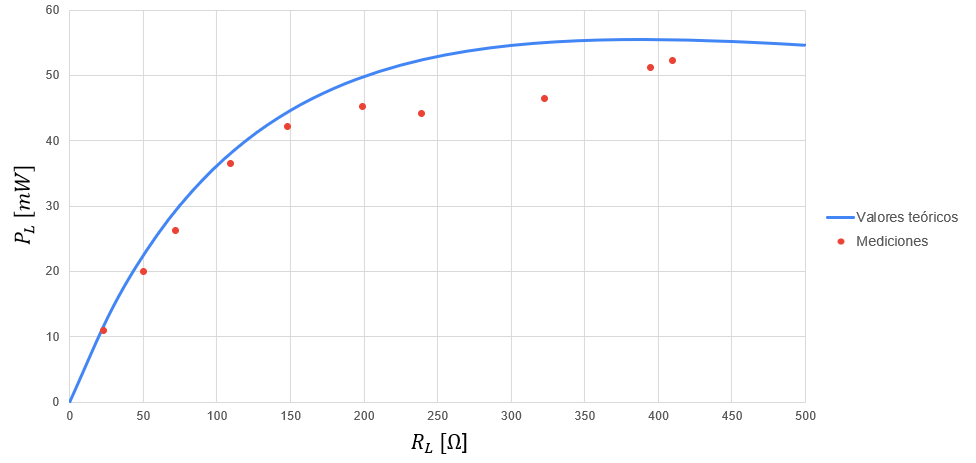
\includegraphics[width=1\textwidth]{graficoPotencia.png}
                \caption{Potencia $P_L$ disipada por el resistor variable $R_L$ en función del valor del mismo.}
                \label{fig:graficoTransferenciaPotencia}
            \end{figure}

            \quad Se puede observar en la tabla que el valor de la máxima potencia disipada por el resistor se corresponde con el valor de $ 360 \Omega $ del mismo.

            \subsubsection{Análisis}
            \quad Se puede observar que los valores teóricos y los medidos son lo suficientemente cercanos para confirmar 
            la validez del valor de teórica de la resistencia de carga $R_L$ que maximiza la potencia disipada.
            Aún así, se debe remarcar que la desviación que hay en la práctica se puede deber a la precisión del multímetro utilizado como también la del osciloscopio
            y por supuesto, a la tolerancia de las resistencias utilizadas en el circuito (5\%).
    %%%Conclusiones%%%
    \section{Conclusiones}

    \quad A lo largo del desarrollo del trabajo práctico, se verificó experimentalmente
     la aplicabilidad de los teoremas de Thévenin y Norton. Además, se adquirió experiencia 
     fundamental en el manejo adecuado de instrumentos de medición y montaje de circuitos 
     eléctricos sobre una protoboard. Como resultado de esta práctiva, se comprobó la efectividad 
     del teorema de máxima transferencia de potencia identificando la resistencia de carga óptima.

    %%%Anexos%%%
    \section{Anexos}

\end{document}